\documentclass{beamer}

\usepackage{hyperref}

\usetheme{Marburg}

\title{Maintainable Embedded Linux Solutions}
\author{Thomas Irgang \and Simone Weiß}
\institute{EASTERHEGG 2024 - RABBIT PROTOTYPING}
\date{March 31, 2024}
\titlegraphic{
    
\includegraphics[width=2cm]{assets/logo.png}
}

\newcommand\pro{\item[$+$]}
\newcommand\con{\item[$-$]}

\begin{document}

\begin{frame}
    \titlepage
\end{frame}

\section{Why Linux?}

\begin{frame}{Do I need Linux for my project?}
	\begin{tabular}{cccc}
	&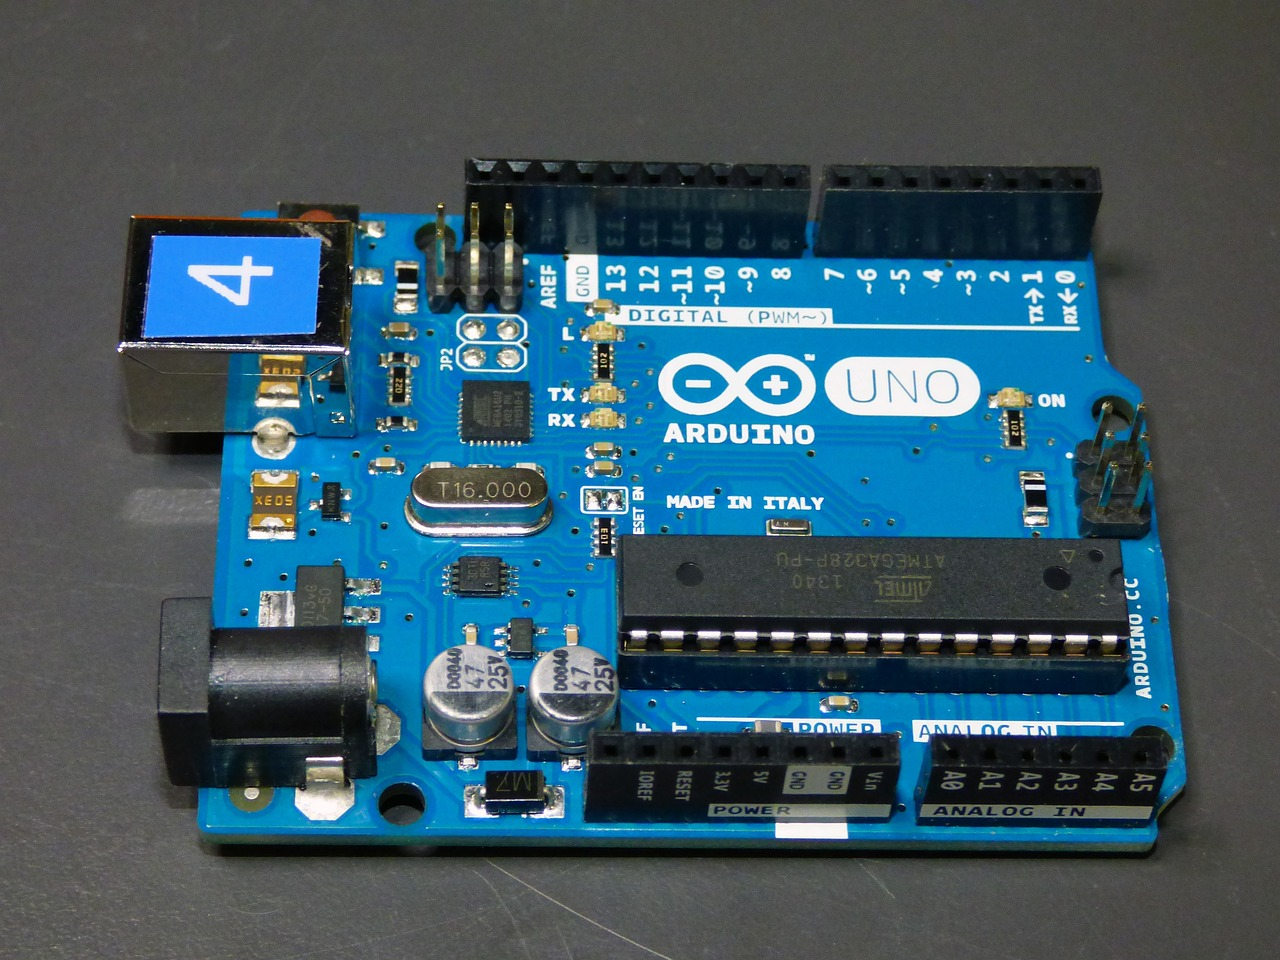
\includegraphics[width=1.9cm]{assets/Pixabay_Arduino_integrated-circuit-441289_1280.jpg} &
	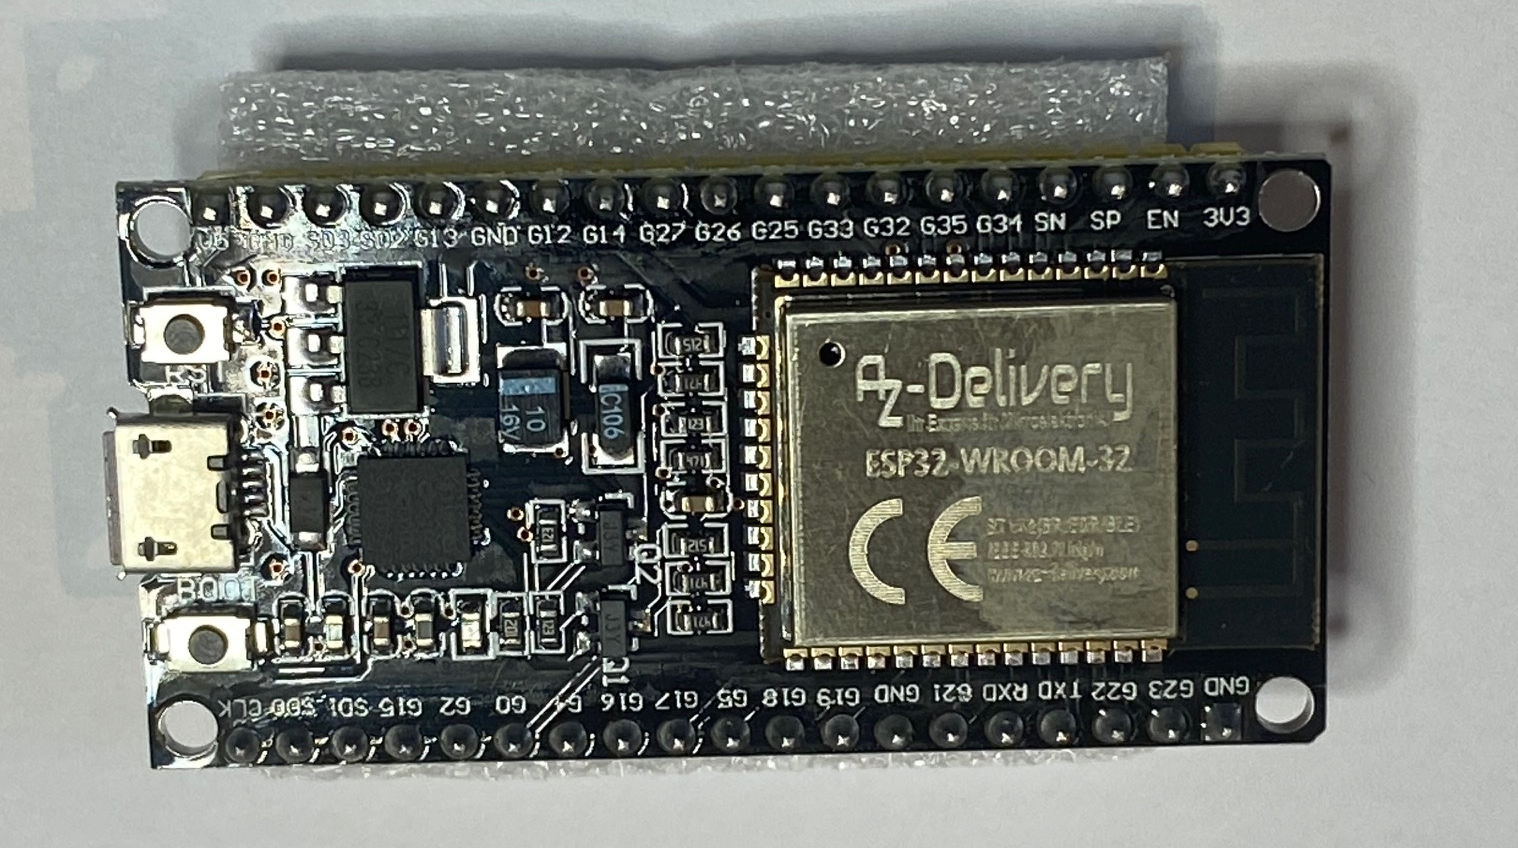
\includegraphics[width=1.9cm]{assets/ESP32.png} & 
	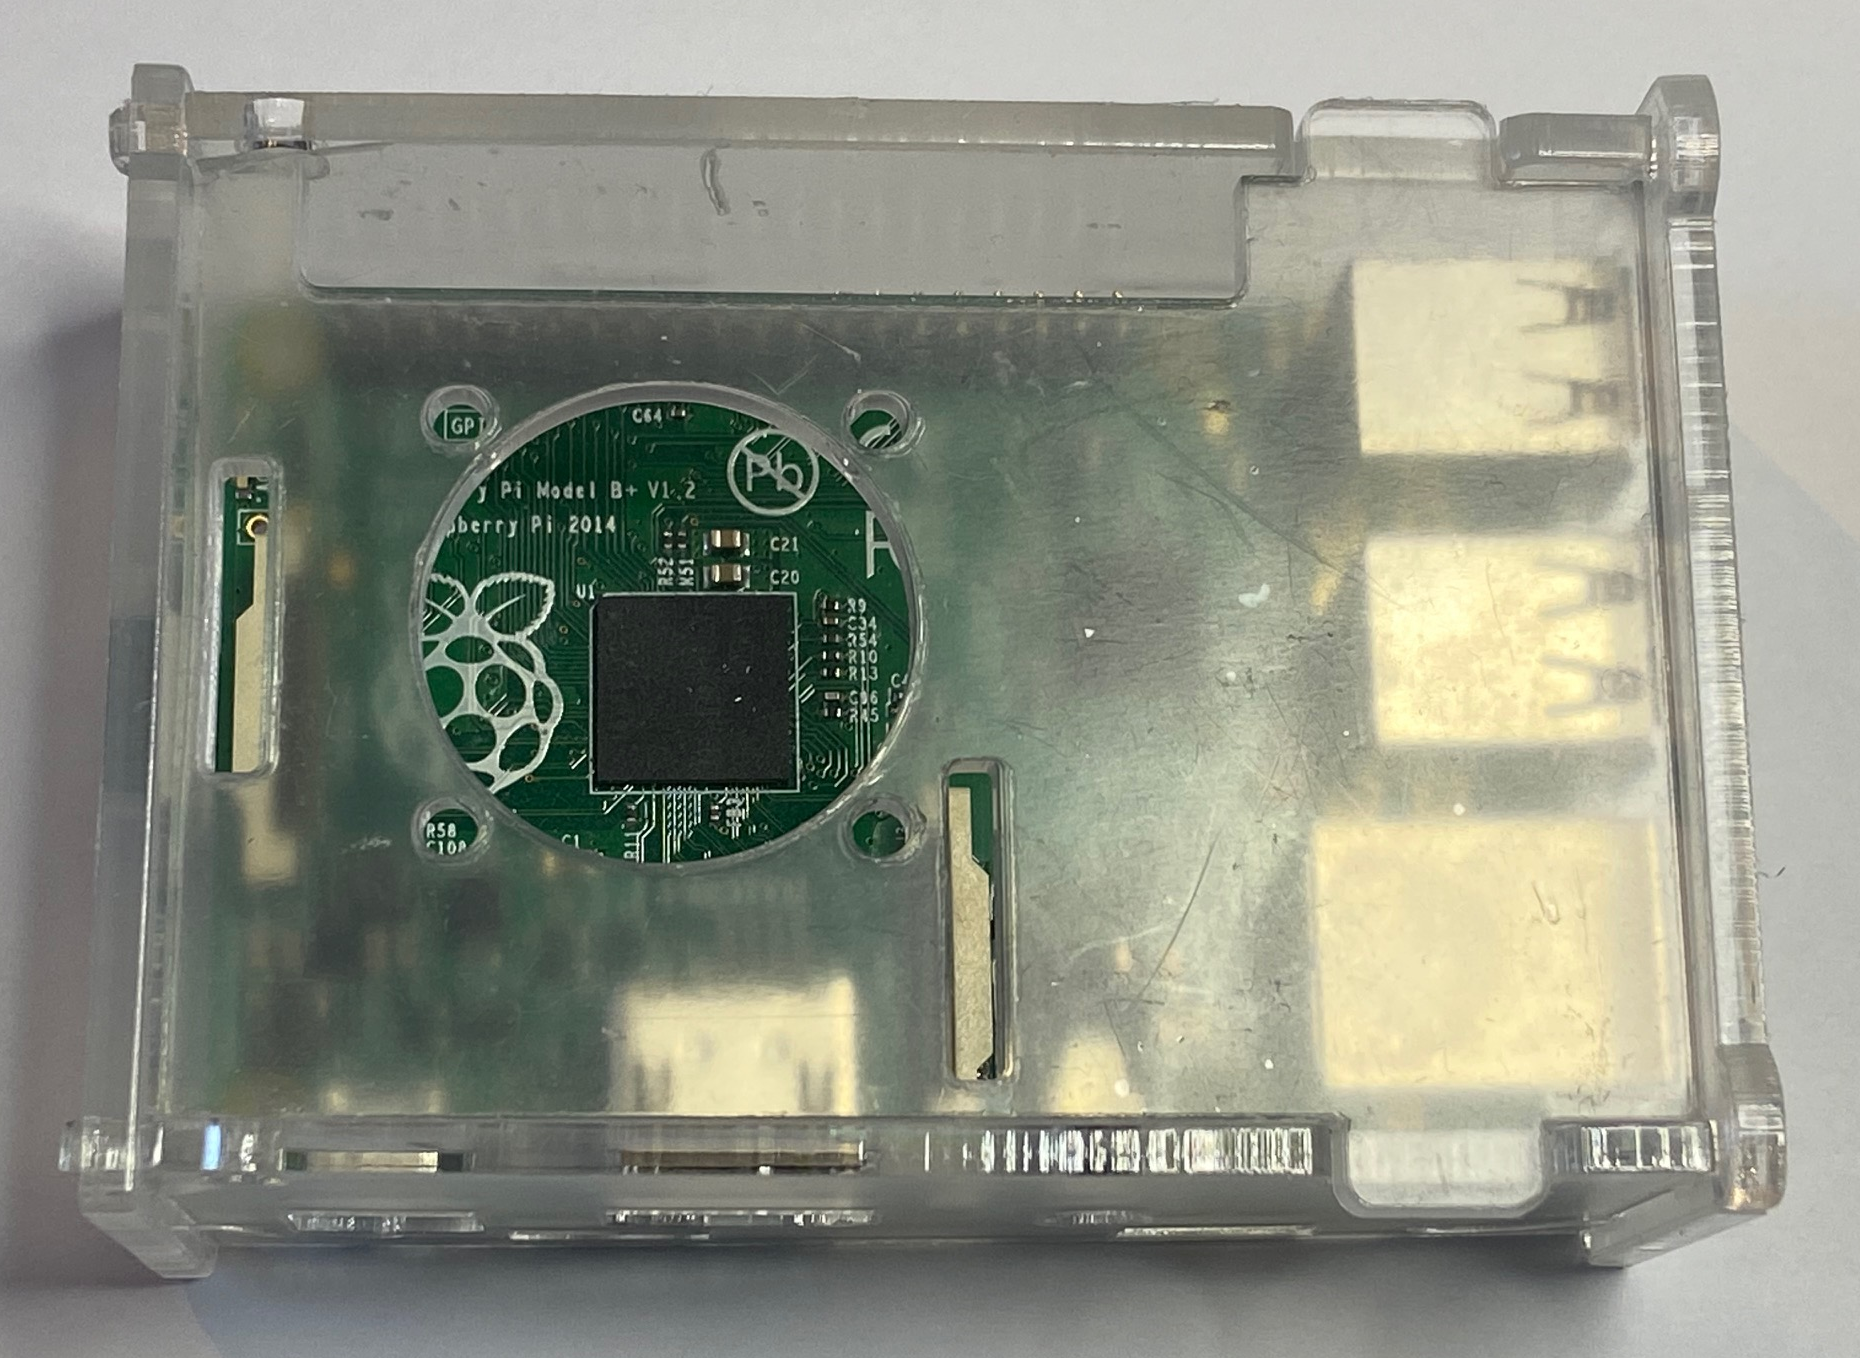
\includegraphics[width=1.9cm]{assets/Raspberry_Pi.png} \\
	&\textbf{Arduino} & \textbf{ESP32 FreeRTOS} & \textbf{SBC Linux} \\
	real-time & + &  + & - \\
	energy & + & o & - \\
	UI & - & - & + \\
	IO & - & o & + \\
	CPU & - & o & + \\
	\end{tabular}
\end{frame}

\begin{frame}{What's the life-time of my project?}
	\begin{columns}
    \column{0.33\textwidth}
        \centering
        \textbf{Experiment}
        \begin{itemize}
        		\item few months
        		\item no maintenance
        		\item some reusability
        \end{itemize}
    \column{0.33\textwidth}
        \centering
        \textbf{Media-Center}
        \begin{itemize}
        		\item some years
        		\item typical IT distribution maintenance
        		\item no reusability needed
        \end{itemize}
    \column{0.34\textwidth}
        \centering
        \textbf{Home Automation}
        \begin{itemize}
        		\item more than 15 years
        		\item maintenance and upgrades
        		\item reusability for mid-term upgrade needed
        \end{itemize}
    \end{columns}
\end{frame}

\section{Embedded Linux}


\begin{frame}{The "golden image" approach}
	\begin{columns}
    \column{0.5\textwidth}
        \centering
        \begin{itemize}
        		\item starting from an existing Linux image, e.g. Raspberry Pi OS,
        		\item install additional required tools,
        		\item and configure the tools
        		\item and the Linux image.
        \end{itemize}
    \column{0.5\textwidth}
        \centering
        \begin{itemize}
        		\pro easy approach
        		\pro maintained by base distribution
        		\con solution and base distribution are mixed
        		\con maintenance out of control
        		\con no support for variants
        		\con huge amount of not needed software
        \end{itemize}
    \end{columns}
\end{frame}

\begin{frame}{The source build toolkit approach}
	\begin{columns}
    \column{0.5\textwidth}
        \centering
        \begin{itemize}
        		\item Yocto or Buildroot
        		\item build all packages from source
        		\item using project specific config and patches
        \end{itemize}
    \column{0.5\textwidth}
        \centering
        \begin{itemize}
        		\pro optimal solution possible
        		\pro minimized amount of resources
        		\pro solution separated and reusable
        		\pro support for variants
        		\con learning curve
        		\con high maintenance effort
        \end{itemize}
    \end{columns}
\end{frame}

\begin{frame}{The remix distribution approach}
	\begin{columns}
		\column{0.5\textwidth}
		\centering
		\begin{itemize}
			\item solution-specific remix of existing distribution
			\item build a custom image using the binary packages of the base distribution
		\end{itemize}
		\column{0.5\textwidth}
		\centering
		\begin{itemize}
			\pro low maintenance effort
			\pro lower amount of resources
			\pro solution separated and reusable
			\pro support for variants
			\con learning curve
			\con limited optimization
		\end{itemize}
	\end{columns}
\end{frame}

\section{The source build toolkit}

\begin{frame}{Tools for source builds}
	\begin{tabular}{c|ccc}
		& \textbf{Yocto} & \textbf{Buildroot}  \\
		\hline
		target & Embedded Image & Debian remix \\ 
		format & deb, rpm, arch & none \\
		cross img & yes & yes \\
		cross pkg & yes & no \\
		compiler & yes & yes \\
	\end{tabular}
\end{frame}

\subsection{Kiwi-ng}

\begin{frame}{Yocto}
	\begin{itemize}
		\item Yocto 
	\end{itemize}
	\begin{definition} 
		Provides Metadata (recipes, configuration, data how things are built), BitBake (buildsystem) to build a custom embedded Linux distribution. It also provides Poky as a reference distribution.
	\end{definition}
	\begin{itemize}
		\item Will build packages and images based on recipes and configuration
		\item Metadata is using Bash and Python
		\item Docs: \url{https://docs.yoctoproject.org/}
		\item Source: \url{git://git.yoctoproject.org/poky}
	\end{itemize}
\end{frame}

\begin{frame}{Yocto: Raspberry Pi image}
	\begin{itemize}
		\item Source: \href{https://github.com/OSInside/kiwi-descriptions/tree/main/ubuntu/aarch64/ubuntu-jammy-rpi}{Github}
		\item based on Poky
		\item Steps:
		\begin{itemize}
			\item install \url{pip3 install kas}
			\item get kas.yml
			\item run kas build
			\item copy image to SD card
		\end{itemize}
		\item more details on \href{https://github.com/tomirgang/eh21_maintainable_linux/tree/main/examples/first_build_rpi4/yocto}{Github}
	\end{itemize}
\end{frame}

\section{Remixing a distribution}

\begin{frame}{Tools for building a remix distribution}
	\begin{tabular}{c|ccc}
		& \textbf{Elbe} & \textbf{Debos} & \textbf{Kiwi-ng} \\
		\hline
		target & Embedded Image & Debian remix & Linux remix \\ 
		format & deb & deb & deb, rpm, arch \\
		cross img & yes & yes & yes \\
		cross pkg & yes & no & no \\
		compiler & yes & no & no \\
	\end{tabular}
\end{frame}

\subsection{Kiwi-ng}

\begin{frame}{Kiwi-ng}
	\begin{itemize}
		\item Appliance builder
	\end{itemize}
	\begin{definition} 
		An appliance is a ready to use image of an operating system including a pre-configured application for a specific use case. 
	\end{definition}
	\begin{itemize}
		\item Supports all major package managers
		\item Image description using XML and config scripts
		\item Docs: \url{https://osinside.github.io/kiwi/}
		\item Source: \url{https://github.com/OSInside/kiwi}
	\end{itemize}
\end{frame}

\begin{frame}{Kiwi-ng: Raspberry Pi image}
	\begin{itemize}
		\item Source: \href{https://github.com/OSInside/kiwi-descriptions/tree/main/ubuntu/aarch64/ubuntu-jammy-rpi}{Github}
		\item based on Ubuntu Jammy
		\item Steps:
		\begin{itemize}
			\item install \url{https://pypi.org/project/kiwi/}
			\item install \url{https://pypi.org/project/kiwi-boxed-plugin/}
			\item get image description
			\item run image build
			\item copy image to SD card
		\end{itemize}
		\item more details on \href{https://github.com/tomirgang/eh21_maintainable_linux/tree/main/examples/first_build_rpi4/kiwi-ng}{Github}
	\end{itemize}
\end{frame}

\subsection{Debos}

\begin{frame}{Debos}
	\begin{itemize}
		\item Debian-based OS image builder
	\end{itemize}
	\begin{definition} 
		debos is a tool to make the creation of various Debian-based OS images simpler. While most other tools focus on specific use-cases, debos is more meant as a tool-chain to make common actions trivial while providing enough rope to do whatever tweaking that might be required behind the scene.
	\end{definition}
	\begin{itemize}
		\item Supports only Debian packages
		\item Image description using YAML
		\item Docs: \url{https://pkg.go.dev/github.com/go-debos/debos}
		\item Source: \url{https://github.com/go-debos/debos}
	\end{itemize}
\end{frame}

\begin{frame}{Debos: Raspberry Pi image}
	\begin{itemize}
		\item Source: \href{https://github.com/go-debos/debos-recipes/tree/main/rpi64}{Github}
		\item based on Debian Bullseye
		\item Steps:
		\begin{itemize}
			\item Debian: install debos packages
			\item run image build
			\item copy image to SD card
		\end{itemize}
		\item more details on \href{https://github.com/tomirgang/eh21_maintainable_linux/tree/main/examples/first_build_rpi4/debos}{Github}
	\end{itemize}
\end{frame}

\subsection{Elbe}

\begin{frame}{Elbe}
	\begin{itemize}
		\item Debian-based embedded image builder
	\end{itemize}
	\begin{definition} 
		Debian-based system to generate root filesystems for embedded devices.
	\end{definition}
	\begin{itemize}
		\item Supports only Debian packages
		\item Image description using XML
		\item Docs: \url{https://elbe-rfs.org/docs/sphinx}
		\item Source: \url{https://github.com/Linutronix/elbe}
	\end{itemize}
\end{frame}

\begin{frame}{Elbe: Raspberry Pi image}
	\begin{itemize}
		\item Based on \href{https://github.com/Linutronix/elbe/blob/master/examples/arm64-qemu-virt.xml}{example arm64-qemu-virt}
		\item Steps:
		\begin{itemize}
			\item Debian: install elbe package
			\item prepare the initvm
			\item run the image build
			\item copy image to SD card
		\end{itemize}
		\item more details on \href{https://github.com/tomirgang/eh21_maintainable_linux/tree/main/examples/first_build_rpi4/elbe}{Github}
	\end{itemize}
\end{frame}

\section{Example project}

\subsection{Raspberry PI image}

% simple RPi CLI image

\subsection{Embedded project}

% TOOD more involved example project

\section{Evaluation}

% Yocto

% Raspbian

% comp with kiwi

% comp with debos

% comp with elbe

% evaluation ideas: performnace, maintainability, flexibility, BSP available?

\end{document}
